\documentclass{article}
\usepackage[left=0.5in,right=0.5in,bottom=0.75in,top=0.75in]{geometry}

% Packages
\usepackage{graphicx}
\graphicspath{{../template/results}}
\usepackage{natbib}
\usepackage{hyperref}
\hypersetup{colorlinks=true, citecolor=black, linkcolor=black, urlcolor=cyan}
\usepackage{booktabs}
\usepackage{xcolor}
\definecolor{codebg}{gray}{0.95}
\usepackage{showexpl}
\lstset{
  basicstyle=\ttfamily\small,
  backgroundcolor=\color{codebg},
  explpreset={numbers=none, pos=r}
}
\usepackage{parskip}

% Macros
\input{math-unicode}

% Icons
\usepackage{fontawesome7}
\definecolor{goodcolor}{HTML}{2E7D32}
\newcommand{\xmark}{\textcolor{red}{\faXmark}}
\newcommand{\cmark}{\textcolor{goodcolor}{\faCheck}}
\newcommand{\bad}{\xmark\; \textbf{Bad:}}
\newcommand{\good}{\cmark\; \textbf{Good:}}

% Notes to each other
\newcommand{\pb}[1]{\textcolor{red}{#1}}
\newcommand{\yl}[1]{\textcolor{blue}{#1}}

% Title/author/date
\title{Style guide / Common \LaTeX \, mistakes}
\author{Patrick Breheny \\ Department of Biostatistics \\ University of Iowa}
\date{\today}

% Move title up a bit
\usepackage{titling}
\pretitle{\begin{center} \LARGE \bf}
  \posttitle{\par\end{center}\vskip 0.5em}
\setlength{\droptitle}{-50pt}

\begin{document}

\maketitle

\section{Cross-references and citations}

\subsubsection*{Label naming conventions}

Labels should:

\begin{itemize}
\item be lowercase
\item use hyphens, not spaces or camelCase
\item include a type prefix (\texttt{sec:}, \texttt{fig:}, \texttt{tab:}, \texttt{eq:}, \texttt{thm:}, etc.)
\end{itemize}

\good

\begin{itemize}
\item \verb|\label{sec:methods-derivation}|
\item \verb|\label{fig:simulation-results}|
\item \verb|\label{eq:score-function}|
\end{itemize}

\bad

\begin{itemize}
\item \verb|\label{Section:Methods}|
\item \verb|\label{simulationResults}|
\item \verb|\label{Table 1}|
\end{itemize}

\subsubsection*{Use \texttt{\textbackslash eqref} for equations}

When referring to an equation, use \verb|\eqref{eq:score-function}|, not \verb|\ref{eq:score-function}|.

\good

\begin{LTXexample}
equation~\eqref{eq:score-function}
\end{LTXexample}

\bad

\begin{LTXexample}
equation~\ref{eq:score-function}
\end{LTXexample}

The eqref version formats the reference as it appears in the actual equation (here, that's with parentheses, but the point is that if you change how equations look, the reference will always match the equation).

\begin{equation}
  \label{eq:score-function}
  u(\bb) = \X \tp \y - \X \tp \X \bb
\end{equation}

\subsubsection*{Use nonbreaking spaces in references}

Use \verb|Section~\ref{sec:methods}|, not \verb|Section \ref{sec:methods}|. The \verb|~| prevents awkward line breaks.

\subsubsection*{Where to put citations?}

This can be complicated. In general, citations should go at the end of a sentence:
\begin{quote}
Penalized regression methods are widely used in high-dimensional settings \citep{Hastie2009,Zou2005}.  
\end{quote}
Every once in a while, the structure of a sentence requires a mid-sentence citation:
\begin{quote}
The lasso induces sparsity \citep{Tibshirani1996}, whereas ridge regression shrinks coefficients continuously \citep{Hoerl1970}.  
\end{quote}
In that sentence, if you were to put both citations at the end, it would be ambiguous and confusing. But try to do this only when absolutely necessary, because it makes sentences less readable:
\begin{quote}
The lasso \citep{Tibshirani1996} is widely used in high-dimensional regression \citep{Hastie2009} and has inspired numerous extensions \citep{Zou2005,Fan2001}.  
\end{quote}
This sentence is choppy and hard to parse.

\subsubsection*{\texttt{\textbackslash citep} versus \texttt{\textbackslash citet}}

Use \verb|\citep{}| for parenthetical citations and \verb|\citet{}| when the author name appears grammatically in the sentence.

\good

\begin{LTXexample}
Several approaches have been proposed
\citep{Fan2001, Zou2005}. \\

\citet{Zou2005} introduced the adaptive
lasso.
\end{LTXexample}

\bad

\begin{LTXexample}
In \citep{Zou2005}, the adaptive lasso was
proposed. \\

Zou \citep{Zou2005} proposed the adaptive
lasso.
\end{LTXexample}

\subsubsection*{Incorrect capitalization in BibTex}

BibTeX styles often convert article titles to sentence case. Braces protect capital letters and acronyms that must remain capitalized.

\good

\begin{center}
\begin{minipage}{0.46\textwidth}
\begin{lstlisting}
title = {Analysis of {RNA}-Seq Data}
\end{lstlisting}
\end{minipage}
\hfill
\begin{minipage}{0.46\textwidth}
  \vspace{0.1em}
  \fbox{Analysis of RNA-seq data}
\end{minipage}
\end{center}

\bad

\begin{center}
\begin{minipage}{0.46\textwidth}
\begin{lstlisting}
title = {Analysis of RNA-Seq Data}
\end{lstlisting}
\end{minipage}
\hfill
\begin{minipage}{0.46\textwidth}
  \vspace{0.1em}
  \fbox{Analysis of rna-seq data}
\end{minipage}
\end{center}

\section{Mathematical writing and typesetting}

\subsubsection*{General advice}

\begin{itemize}
\item Avoid double-subscripts like $A_{n_i}$
\item Avoid introducing symbols for quantities you only use once
\item When defining something, it is usually a good idea to give it both a technical and conceptual definition. For example: Let $L(\beta) = \sum_i \ell_i(\beta)$ denote the log-likelihood, which measures how well the value $\beta$ agrees with the data.
\end{itemize}

\subsubsection*{Math mode is for mathematical symbols, not ordinary text}

Unadorned letters in math mode are interpreted as variables. If you write \verb|AIC| in math mode, this will be typeset as $AIC$: the variable $A$ times the variable $I$ times the variable $C$. If you need AIC in an equation, use \verb|\text{AIC}|, \verb|\text{CV}|, and so on.

Similarly, don't write \verb|log|, \verb|exp|, \verb|max|, and so on. There are precisely defined commands for all these mathematical operators that preserve correct spacing and typography: \verb|\log|, \verb|\exp|, \verb|\max|.

\good

\begin{LTXexample}
$ \text{AIC} = -2\ell + 2p $ \\
$ \exp x = \max_y \log y $
\end{LTXexample}

\bad

\begin{LTXexample}
$ AIC = -2\ell + 2p $ \\
$ exp x = max_y log y $
\end{LTXexample}

\subsubsection*{Don't type the pipe}

Use \verb|\mid|, \verb|\abs|, and \verb|\norm|. Never type \verb/|/ directly.

\good

\begin{LTXexample}
$ \abs{x} > \Pr(\norm{\y} \mid z $)
\end{LTXexample}

\bad

\begin{LTXexample}
$ |x| > \Pr(||\y|| | z $)
\end{LTXexample}

\subsubsection*{Equations are part of the sentence}

Equations should follow ordinary punctuation rules.

\begin{LTXexample}
If the equation ends a sentence, it needs a
period, like this:

$$ L(\beta) = \sum_{i=1}^n \ell_i(\beta). $$

If the equation ends a clause, as in

$$ L(\beta) = \sum_{i=1}^n \ell_i(\beta), $$

it needs a comma.
\end{LTXexample}

Displayed equations are not punctuation-free objects floating outside the grammar of the paragraph.

\section{Typography and punctuation}

\subsubsection*{Dashes and hyphens}

\begin{itemize}
\item Use a single \verb|-| for hyphenated words
\item Use two dashes \verb|--| for ranges and relationships
\item Use three dashes \verb|---| for interruptions and emphasis
\end{itemize}

\begin{LTXexample}
Brad Efron is a well-known statistician. \\
The bias--variance tradeoff is shown on
pages 10--15. \\
Bias --- while traditionally considered bad ---
can often be useful.
\end{LTXexample}

\subsubsection*{LaTeX requires directional quotes}

\good

\begin{LTXexample}
``quoted text''
\end{LTXexample}

\bad

\begin{LTXexample}
"quoted text"
\end{LTXexample}

Note that the quotes on the left are backwards in the ``bad'' example.

\section{Miscellaneous}

\subsubsection*{Do not ignore LaTeX errors and warnings}

A document should compile cleanly before you share it with any collaborators. Almost all warnings indicate genuine problems: undefined references, doubly-defined references, missing citations, overfull boxes, package conflicts, etc. It doesn't matter if the PDF looks OK to you --- the warning is there for a reason and usually indicates a serious underlying problem that will only snowball, growing worse and worse the longer you take to fix it.

\subsubsection*{Don't say ``real data''}

Never title a section ``Real Data''. This tells the reader nothing about the application. Every dataset used in a scientific study is real. The purpose of an application is to demonstrate how the method addresses a substantive scientific question. Use descriptive titles and engage with the scientific context of the analysis.

\good

\begin{quote}
In Section 5, we apply our method to a gene expression study of breast cancer patients.
\end{quote}

\bad

\begin{quote}
In Section 5, we apply our method to real data.
\end{quote}

\section{Figures and tables}

Every figure and table should:

\begin{itemize}
\item have a caption
\item have a label
\item be referenced in the text (using the label, not something like ``see the figure below'')
\end{itemize}

\subsubsection*{Figures}

The call to \verb|\includegraphics{}| should not include the directory path --- only the file name. The path to the directory where the figures are located should be set with \verb|\graphicspath{}| in the preamble; see the template for an example.

\begin{LTXexample}
\begin{figure}
  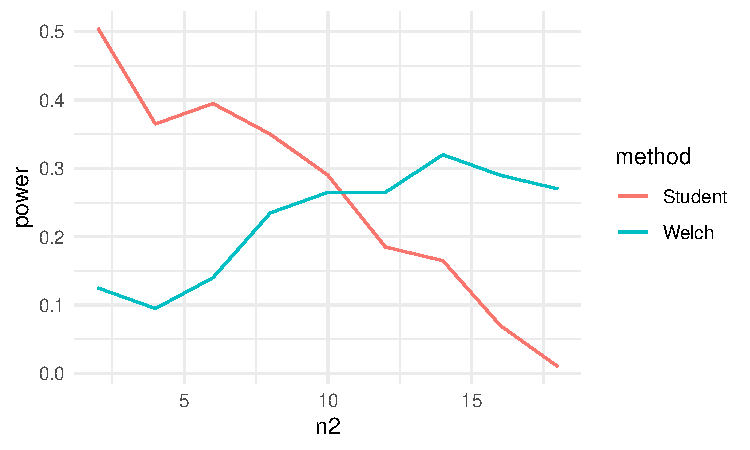
\includegraphics[width=\linewidth]{power}
  \caption{Student's $t$-test (which assumes
  equal variance) suffers from a lack of power
  when the large-variance group is has more
  observations than the small-variance group.}
  \label{fig:power}
\end{figure}
\end{LTXexample}

\subsubsection*{Tables}

\begin{enumerate}
  \item Use \verb|\toprule|, \verb|\midrule|, and \verb|\bottomrule| (from the \texttt{booktabs} package)
  \item Never use vertical rules.
  \item Align numbers consistently.
  \item Report only enough digits to convey meaningful information. No one could possibly care that the type 1 error rate was 0.1121 instead of 0.11. Every digit must justify its existence. Extra digits consume space, distract the reader, and almost never affect the scientific conclusion. When in doubt, round more aggressively.
\end{enumerate}

For more on how to lay out a professional-looking table, see the \href{https://mirrors.ibiblio.org/pub/mirrors/CTAN/macros/latex/contrib/booktabs/booktabs.pdf}{booktabs documentation}.

\begin{LTXexample}
\begin{table}
\centering
\caption{Type 1 error for Student and Welch
$t$-tests. Ratio ($n_1:n_2$) displays the sample
size of the low-variance and high-variance
groups (low-variance first). Student's test
suffers from inflated Type I error when the
small-variance group is larger.}
\label{tab:error-rate}

\begin{tabular}{lrr}
\toprule
Ratio & Student & Welch\\
\midrule
4:16 & 0.03 & 0.06\\
10:10 & 0.05 & 0.05\\
16:4 & 0.14 & 0.06\\
\bottomrule
\end{tabular}

\end{table}
\end{LTXexample}

\subsubsection*{Tables should be reproducible}

The above example is somewhat misleading: in most cases, you shouldn't be directly typing the table contents. The table contents should be automatically generated, typically from \verb|knitr::kable("latex", booktabs = TRUE)|, then use \verb|\input{}|, as in the following, where the output from \verb|kable()| has been saved as \verb|t-tab.tex|:

\begin{LTXexample}
\begin{table}
\centering
\caption{Type 1 error for Student and Welch
$t$-tests. Ratio ($n_1:n_2$) displays the sample
size of the low-variance and high-variance
groups (low-variance first). Student's test
suffers from inflated Type I error when the
small-variance group is larger.}
\label{tab:same-error-rate}
../template/results/error-rate.tex
\end{table}
\end{LTXexample}

The output is exactly the same, but the point is that if you alter or re-run the simulation, the document is guaranteed to track those changes.

\newpage

\bibliographystyle{smallcap}
\bibliography{ref}

\end{document}
